\documentclass{article}

\usepackage[letterpaper, portrait, margin=1.5in]{geometry}

\usepackage{fancyhdr}
\usepackage{ragged2e}
\usepackage{graphicx}
\usepackage{caption}
\usepackage{amsmath}
\usepackage{rotating}

\usepackage{listings}
\usepackage{color}

\definecolor{dkgreen}{rgb}{0,0.6,0}
\definecolor{gray}{rgb}{0.5,0.5,0.5}
\definecolor{mauve}{rgb}{0.58,0,0.82}

\lstset{frame=tb,
  language=Java,
  aboveskip=3mm,
  belowskip=3mm,
  showstringspaces=false,
  columns=flexible,
  basicstyle={\small\ttfamily},
  numbers=none,
  numberstyle=\tiny\color{gray},
  keywordstyle=\color{blue},
  commentstyle=\color{dkgreen},
  stringstyle=\color{mauve},
  breaklines=true,
  breakatwhitespace=true,
  tabsize=4
}

\setcounter{secnumdepth}{1}

\usepackage{chngcntr}
\counterwithin{figure}{section}

\renewcommand*{\thepage}{C\arabic{page}}

\pagestyle{fancy}
\lhead{ACME Robotics}
\chead{\#8367}
\rhead{\ifcontents Contents \else Week \thesection \fi}

\newif\ifcontents
\contentstrue

\makeatletter
\renewcommand{\@seccntformat}[1]{}
\makeatother
\begin{document}

\subsection{Hardware Discussion}
%! Have a team-wide discussion about the next steps for the hardware team.
After the first competition the team's goals were reevaluated. The sorting mechanism was not functional and untested. The lift motor was not correctly mounted and its spool was causing issues. The rake mechanism for the intake used a pulley system that had a tendency to unspool and the REV friction slides were not working correctly, which resulted in each side retracting at different speeds. The team had a meeting to discuss what the next steps were. They listed priorities, such as the lift, intake and the sorting mechanism. These were the things that the team felt were vital to successfully compete in the next competition. The week was spent testing several concepts that the team didn't have time to test before the Burlingame tournament. 

The outcome of the discussion lead to a large change in the overall placement of specific subsystems, resulting in a great deal of CAD redesign. The team ended of changing the placement of the drivetrain's cross members to allow for the correct placement of the lift-motor. The team also realized that the design could be more streamlined and compact, by adding the intake's super-structure to the drivetrain's aluminum side-plates. Along with adding mounting holes for the subsystems that was not previously foreseen.  


\subsection{Sorter Testing}
%!Test the sorter to see if the team needs to reevaluate the sorting process.
Aidan took on the project of testing the sorter. The team didn't have time to incorporate the sorter into the robot before the Burlingame tournament and still needed to be assembled and tested. Aidan and Ashlin tried to assemble the sorter specifically so that it would take up as little space as possible, as seen in Figure \ref{fig:sortertesting}. They did this because there was limited space on the inside of the robot and the sorter, the cartridges, and the lift motor were all competing for this room. After fully assembling the sorter and testing the the team decided it took to much room and they wouldn't pursue it any further.

\begin{figure}
    \centering
    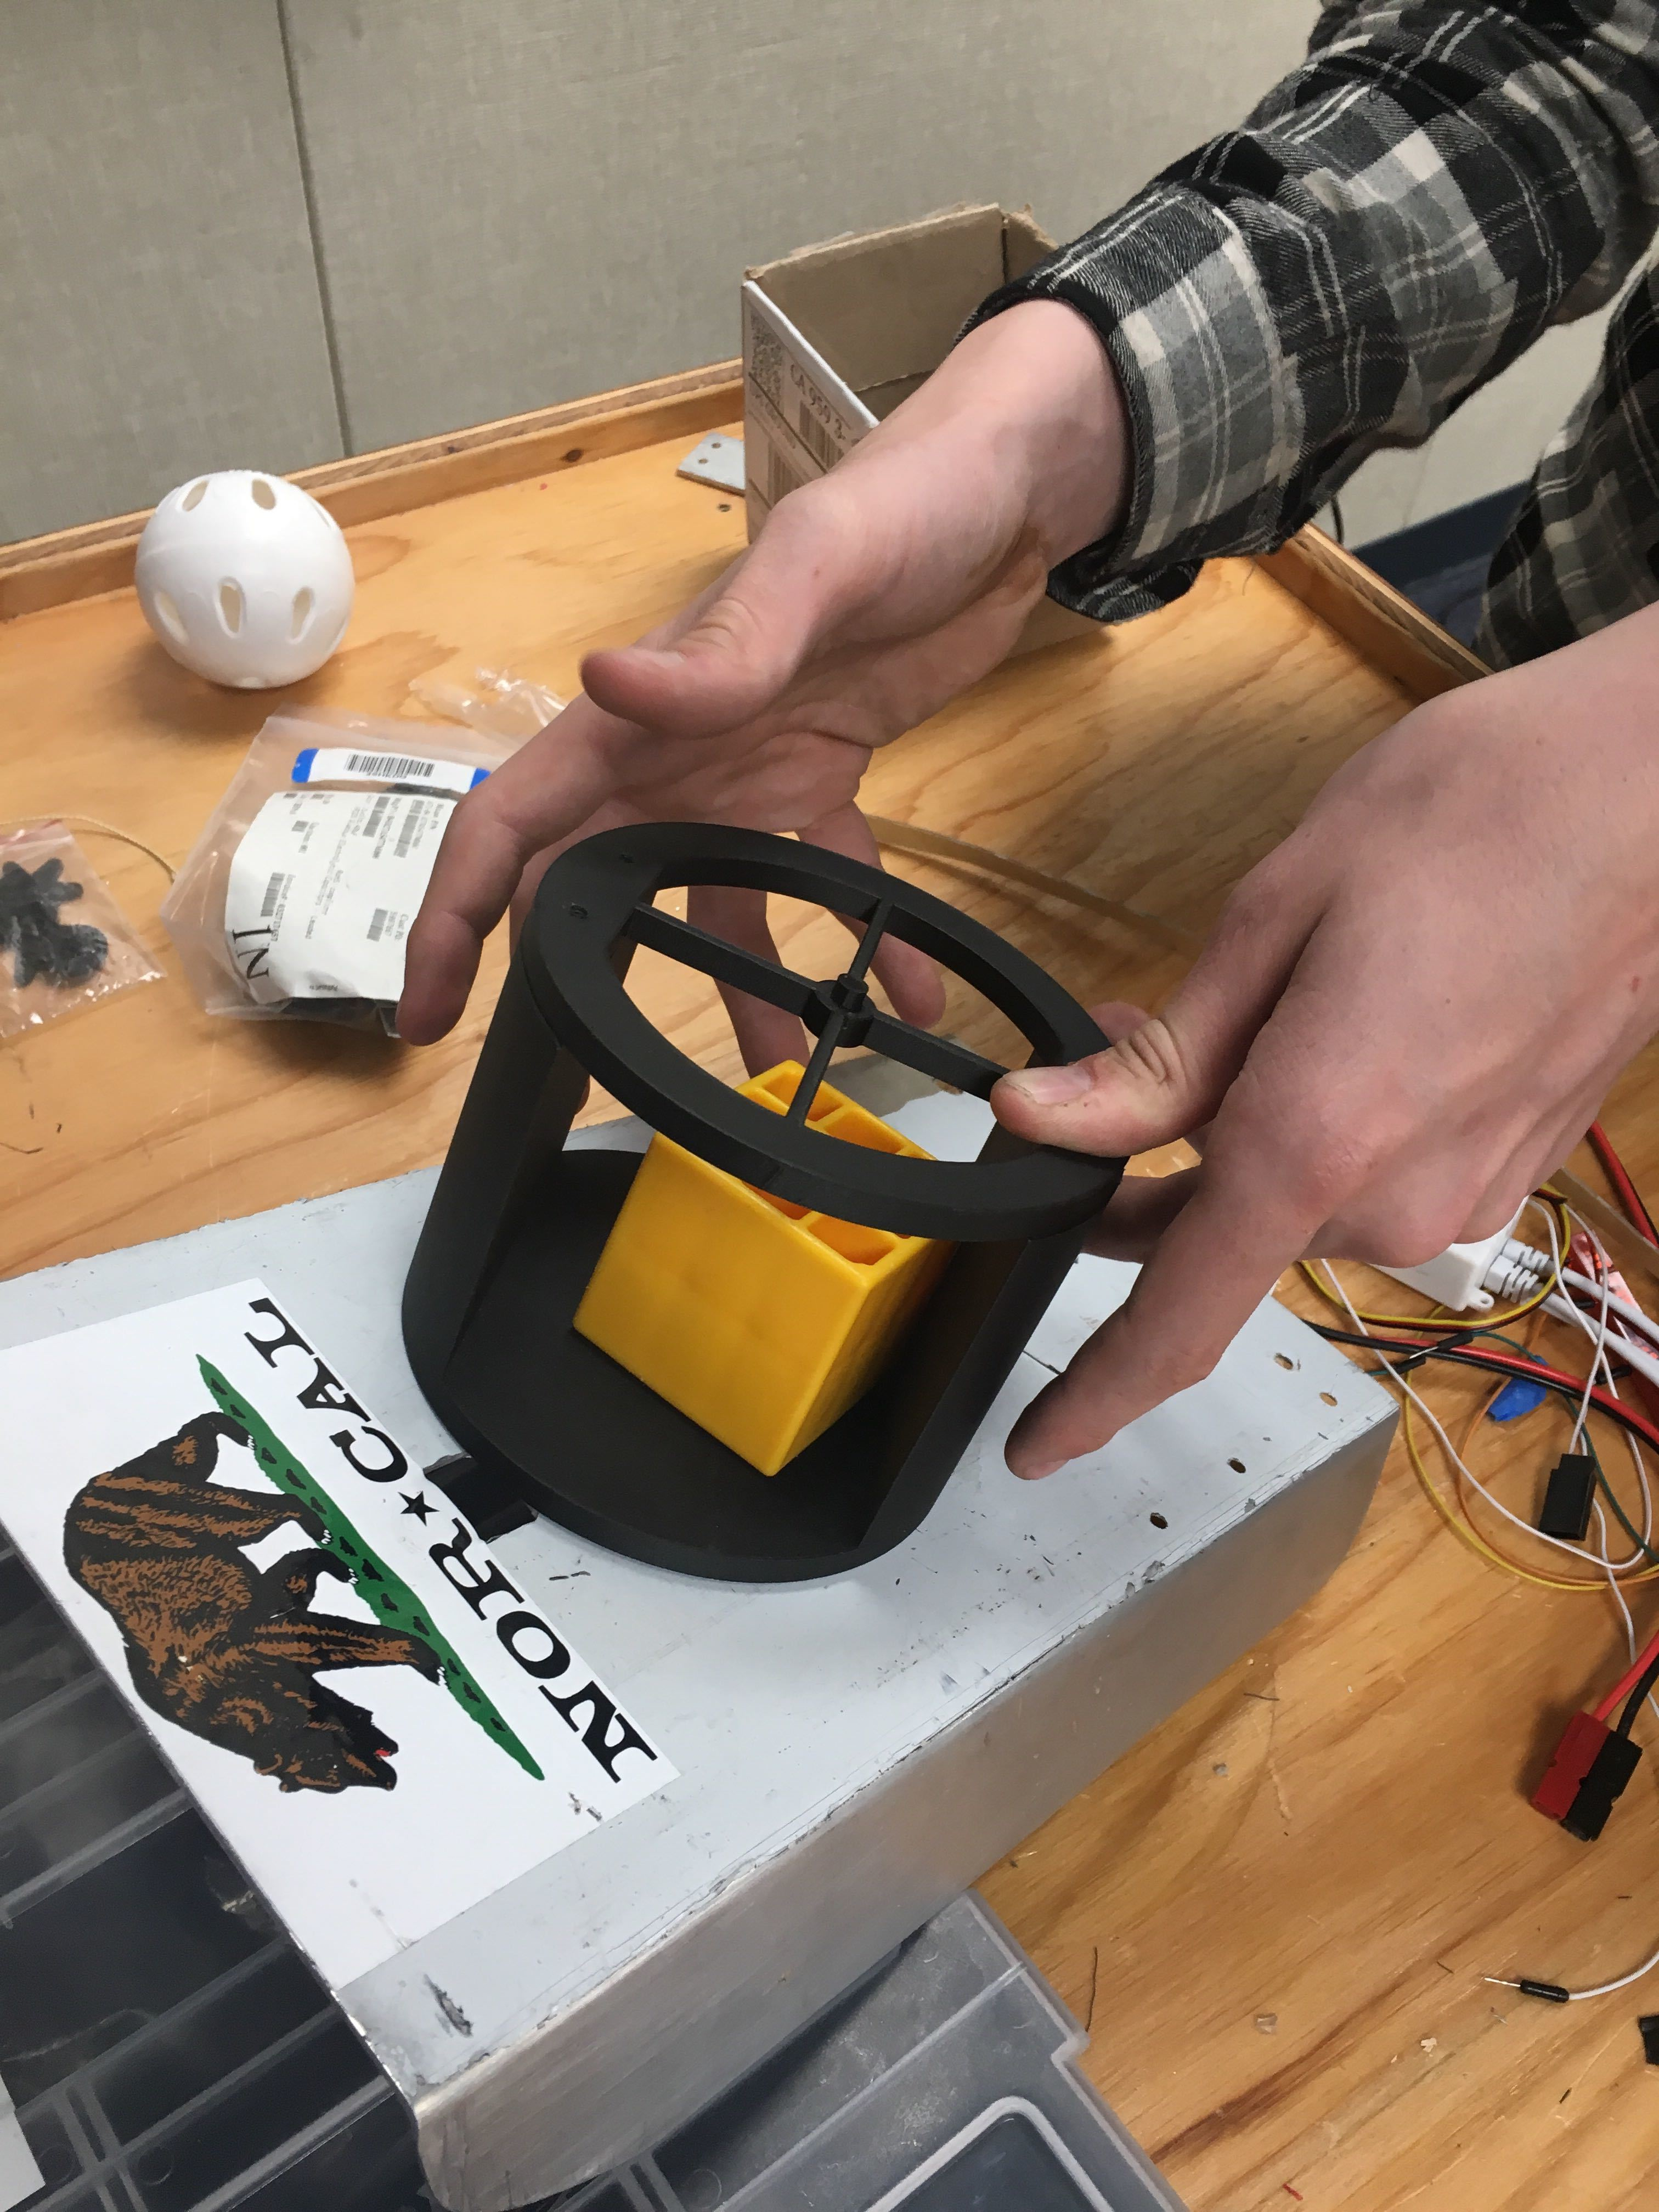
\includegraphics[width=.6 \textwidth]{13_11-26/images/sorting.JPG}
    \caption{Testing the Sorter}
    \label{fig:sortertesting}
\end{figure}

\subsection{Latch Design and Development}
%! Design a latch to mount on the robot that will be used to latch onto the lander.
Ben and Shawn designed the latch to make the robot hang. They used a design where, if the robot was fully turned off, the robot would still latch. They designed it so that the servo pulls the axle back so they robot isn't latched anymore. They then prototyped this design with Tetrix and found that there were problems. Here is the latch on the lander in Figure \ref{fig:latch1}. Then they solved these problems and are going to try to find a way to manufacture a more professional looking latch.

\begin{figure}
    \centering
    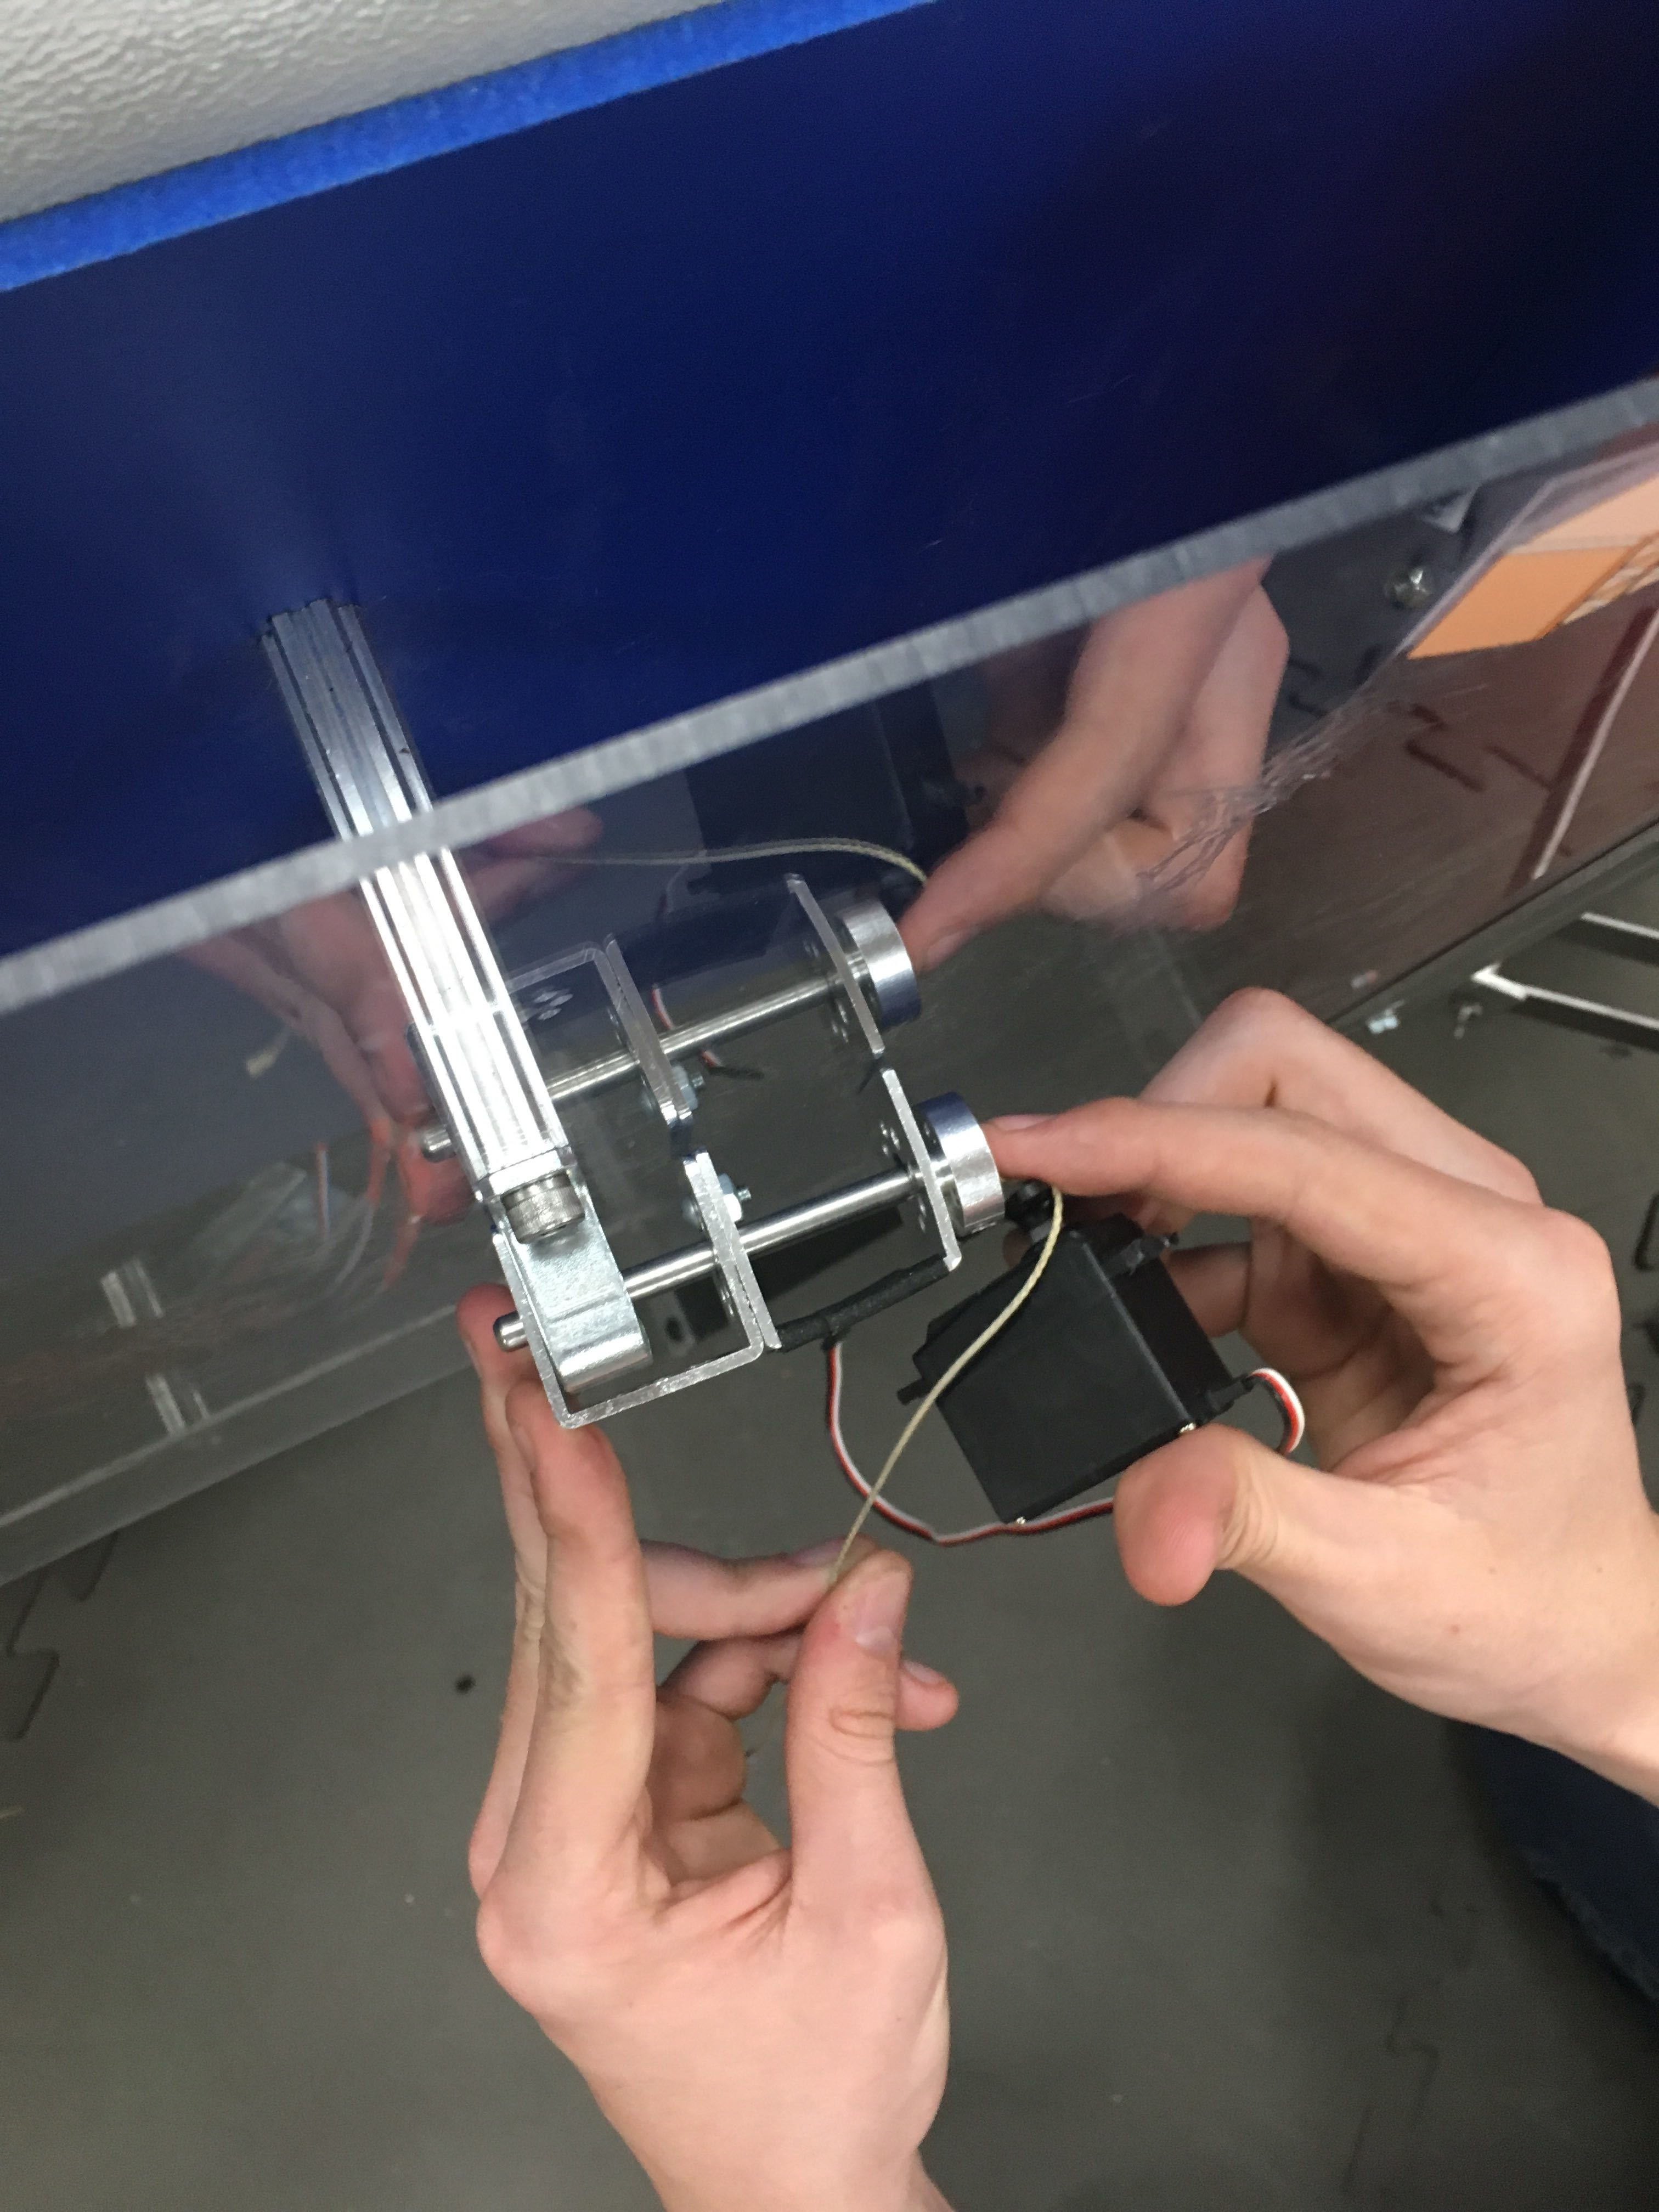
\includegraphics[width=.6 \textwidth]{13_11-26/images/latchservo.JPG}
    \caption{Latch}
    \label{fig:latch1}
\end{figure}


\subsection{Testing of Rev linear slides}
%! Test the REV linear slides the team uses for the rake.
After the team's first qualifier where the rake did not function properly, ACME wanted to do some testing and see what the problem was. The rake system is crucial to ACME's current design so it was important that this was done ASAP. After Jon did some testing with the rake, he found that the problem lay with the Rev linear slides. There was too much friction in the slides and the string was spooled wrong and was causing the slides to move unevenly. He also found that the string had a tendency to become un-spooled. Jon and the rest of the team decided that removing one of the slides might remedy the problem. After Jon tested this some, he found that while somewhat better, the results where still far from satisfactory. This lead Jon to the conclusion that the Rev linear slides would have to be scrapped for some other form of linear motion. Jon then commenced brainstorming, researching, and testing for several other forms of linear motion. Nearly all the options Jon looked into did not fit for what ACME had in mind. For example, drawer slides were too heavy could not reach far to far crater wall. One that did look promising however was X-Rail. Jon thought X-Rail looked promising because it was similar to the Rev linear slides in function but could carry more weight, were sturdier, and used running bearings (making them smoother and removing friction). This made X-Rail the most practical and simple option. After presenting his findings to the team, ACME decided to give X-Rail a try. 

\end{document}
